% Graficas 
\documentclass[12pt]{article}

\usepackage[T1]{fontenc}
\usepackage[utf8]{inputenc}
\usepackage[spanish]{babel}
\usepackage{amsmath}
\usepackage{amssymb, amsfonts, latexsym, cancel}
\usepackage{graphicx}
\usepackage{epstopdf}
\usepackage{float} %Deja el imagen en donde queramos/escribimos. 
\usepackage{subfigure}

\parindent=0cm

\begin{document}
\title{Practica 4 \\ Gráficas}
\author{Rakibul Alam}
\date{}
\maketitle

\tableofcontents

\section{Incluir gráficas externas}

En \LaTeX podemos incluir figuras externas o generadas directamente en \LaTeX \, utilizando algun paquete, algunos de los formatos que podemos utilizar son \textbf{.jpg}, \textbf{.png}, \textbf{.eps} y  \textbf{.pdf}. \\[0.5cm]
Los formatos vectoriales como los son \textbf{.eps} y \textbf{.pdf} son los mas recomendados cuando hacemos graficas en las cuales queremos observar detalles y precision, porque no pierden calidad al aumentar o disminuir su tamano. Y para imagenes en general podemos utilizar los formatos \textbf{.jpg} o \textbf{.png}



\section{Paquetes graphicx}
\begin{center}
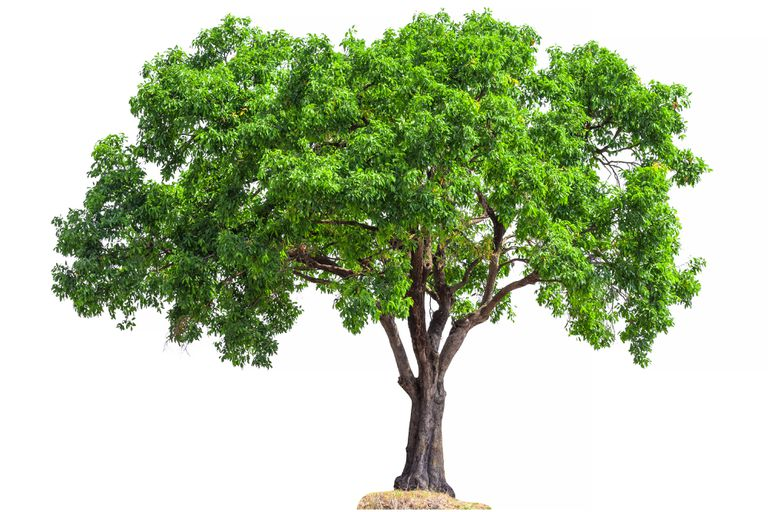
\includegraphics[scale=.2]{figuras/tree.jpg}
\end{center}

\begin{itemize}
\item scale: Escala de la imagen
\item width: Ancho deseado de la imagen en cm. 
\item height: Altura de la imagen en cm. 
\end{itemize}

\begin{center}
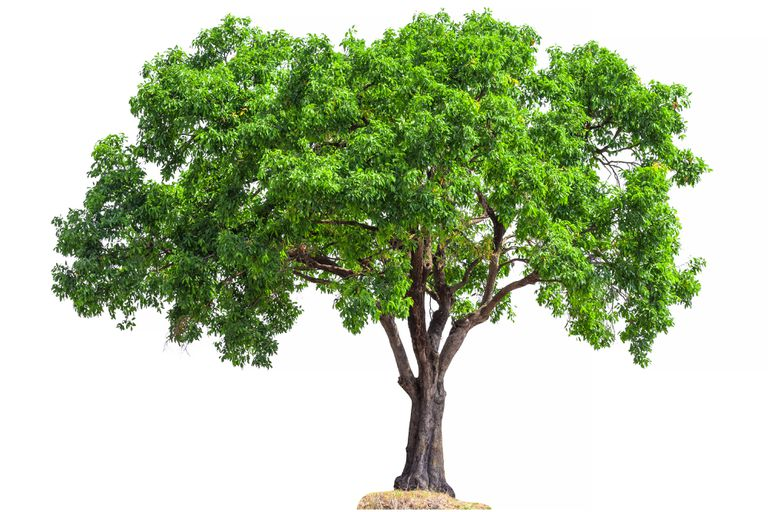
\includegraphics[scale=.3]{figuras/tree.jpg}
\end{center}

\begin{center}
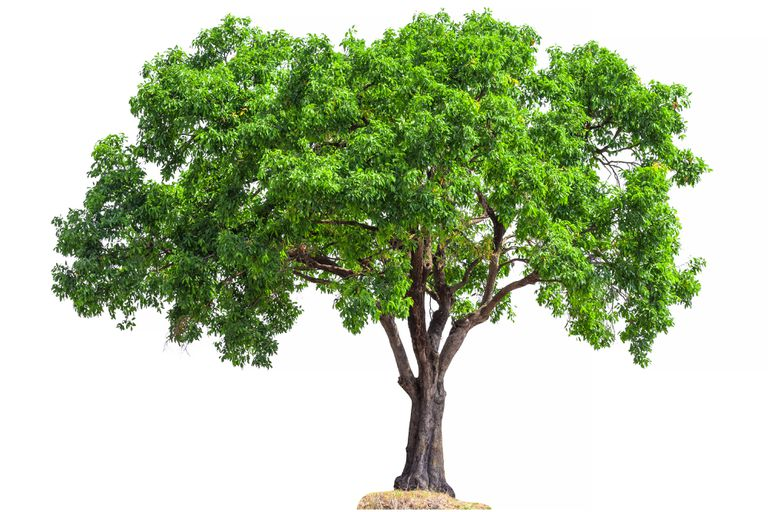
\includegraphics[width = 4cm]{figuras/tree.jpg}
\end{center}

\begin{center}
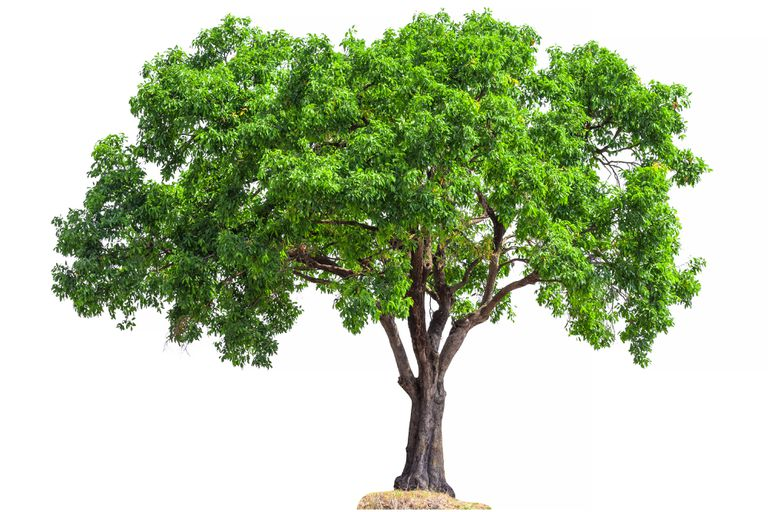
\includegraphics[height = 5cm]{figuras/tree.jpg}
\end{center}

\begin{center}
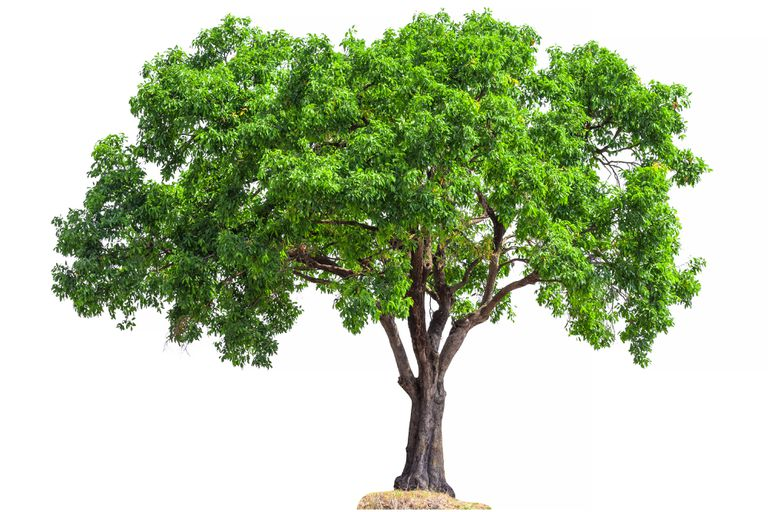
\includegraphics[scale=.1]{figuras/tree.jpg} \quad
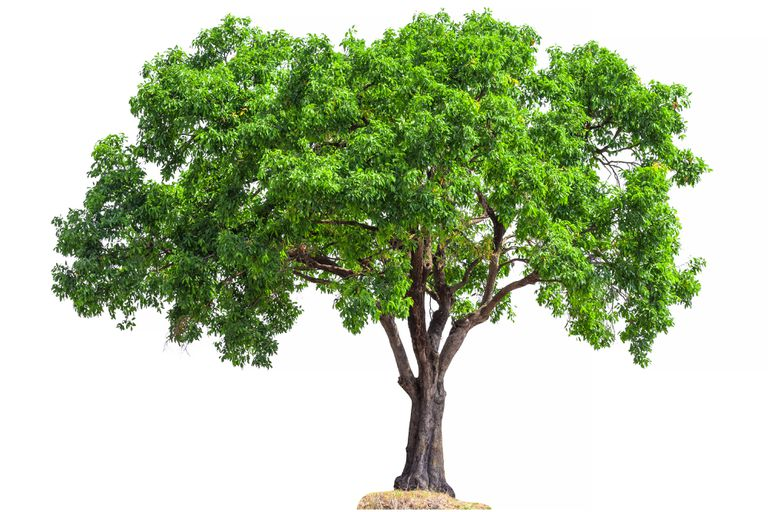
\includegraphics[scale=.15]{figuras/tree.jpg} \quad
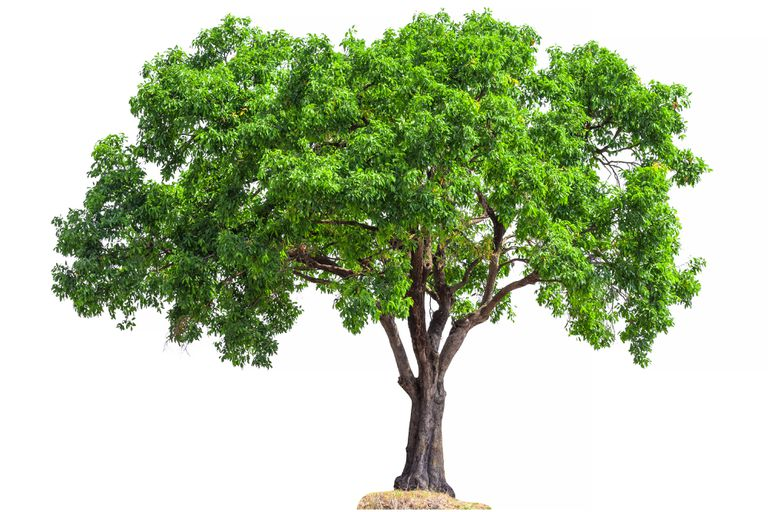
\includegraphics[scale=.2]{figuras/tree.jpg} \quad
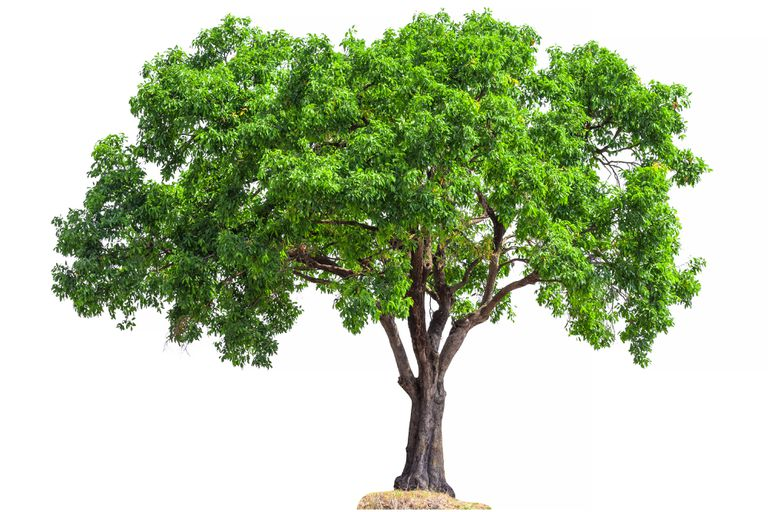
\includegraphics[scale=.25]{figuras/tree.jpg}
\end{center}

%\newpage
\section{Objetos flotantes}

% [!ht] = put the image on the top of the page. 
% [!hb] = put the image on the bottom of the page.

\begin{figure}[!hb]
\centering
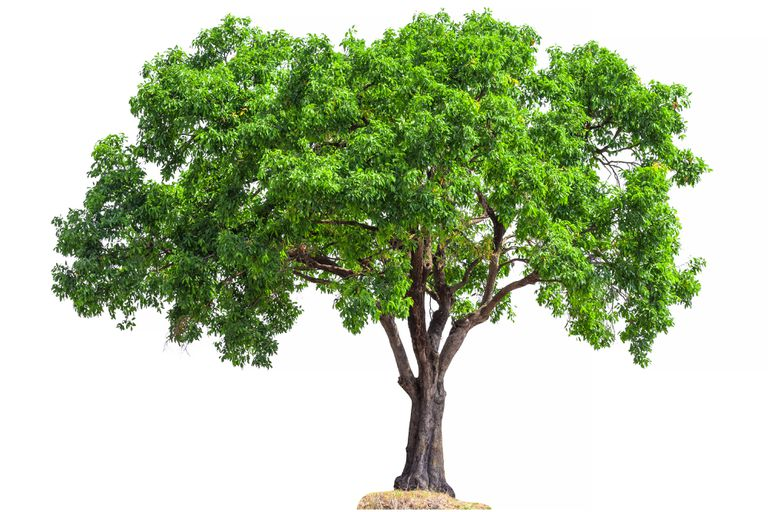
\includegraphics[scale=0.1]{figuras/tree.jpg}
\caption{Imagen a escala 0.1}
\label{figura1}
\end{figure}

\begin{itemize}
\item t: La imagen en la parte superior (top)
\item b: La imagen en la parte inferior (bottom)
\item h: La imagen en el sitio que escribimos (here) 
\end{itemize}

\begin{figure}[H]

\includegraphics[scale=2]{figuras/epsimg.eps}
\caption{Imagen eps}
\label{figura2}
\end{figure}


Aqui estoy hablando de imagenes eps como ea figura \ref{figura2}

\newpage
\subsection{Paquete subfigure}


\begin{figure}[!ht]
\centering
\subfigure[Figura uno]
{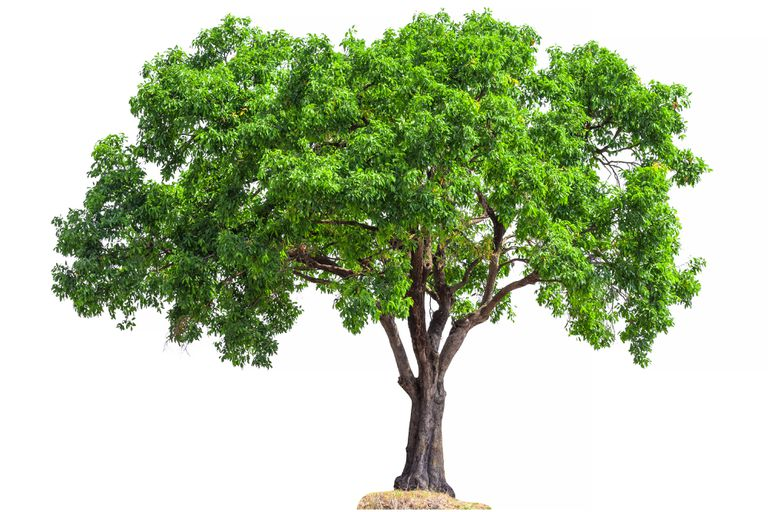
\includegraphics[scale=0.1]{figuras/tree.jpg}}
\quad
\centering
\subfigure[Figura dos]
{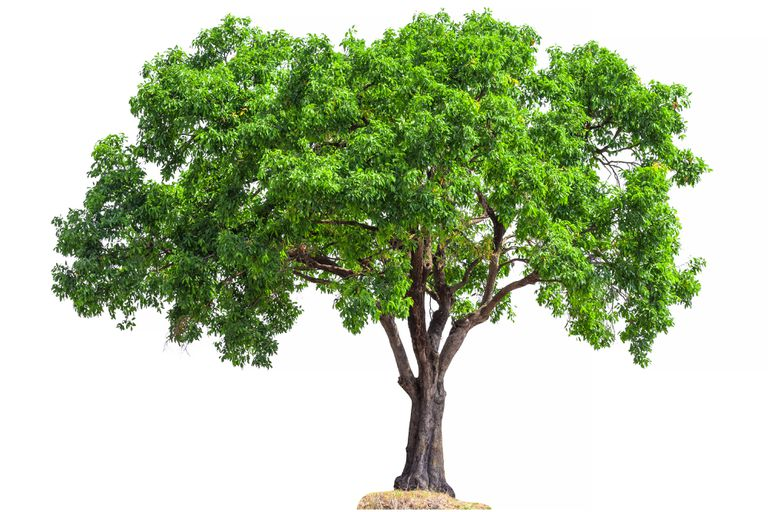
\includegraphics[scale=0.1]{figuras/tree.jpg}}
\quad
\centering
\subfigure[Figura tres]
{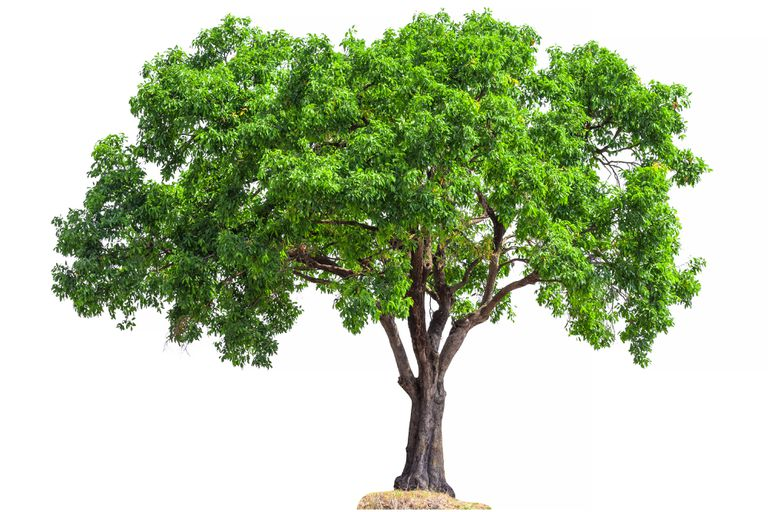
\includegraphics[scale=0.1]{figuras/tree.jpg}}
\caption{Las tree figuras}
\label{3fig}
\end{figure}

Aqui doy ref a los 3 figuras \eqref{3fig}

\begin{figure}[H]
\centering

\includegraphics[scale=3]{figuras/epsimg.eps}
\put(0, 0){\footnotesize{Usando el comando put}}

\caption{Imagen eps}
\label{figura4}
\end{figure}


\end{document}
